\documentclass[article]{jss}
\usepackage[utf8]{inputenc}
\usepackage[nogin]{Sweave}
\usepackage{pdfpages}
\usepackage{xspace}
\usepackage{tikz}
\usetikzlibrary{shapes.geometric, arrows}

\tikzstyle{io} = [trapezium, trapezium left angle=70, trapezium right angle=110, minimum width=3cm, minimum height=1cm, text centered, draw=black, fill=blue!30]
\tikzstyle{process} = [rectangle, minimum width=3cm, minimum height=1cm, text centered, draw=black, fill=orange!30]
\tikzstyle{decision} = [diamond, minimum width=3cm, minimum height=1cm, text centered, draw=black, fill=green!30]
\tikzstyle{arrow} = [thick,->,>=stealth]


\newcommand{\hl}[1]{\textcolor{magenta}{#1}}

%Virker ikke:
%\newcommand{\R}{\proglang{R}\xspace}

\newcommand{\R}[1]{\code{#1}}

%%%%%%%%%%%%%%%%%%%%%%%%%%%%%%
%% declarations for jss.cls %%%%%%%%%%%%%%%%%%%%%%%%%%%%%%%%%%%%%%%%%%
%%%%%%%%%%%%%%%%%%%%%%%%%%%%%%

%% almost as usual
\author{Anne H. Petersen\\Biostatistics\\Department of Public
  Health\\University of Copenhagen \And Claus Thorn Ekstr\o m\\Biostatistics\\Department of Public
  Health\\University of Copenhagen}
\title{\pkg{cleanR}: Maid for Cleaning Datasets in \proglang{R}}

%% for pretty printing and a nice hypersummary also set:
\Plainauthor{Anne H. Petersen, Claus Thorn Ekstr\o m} %% comma-separated
\Plaintitle{{cleanR}: maid for cleaning datasets in R} %% without formatting
\Shorttitle{\pkg{cleanR}: maid for cleaning datasets in R} %% a short title (if necessary)

%% an abstract and keywords
\Abstract{Data cleaning and -validation are the first steps in any
  data analysis, as the validity of the conclusions from the analysis
  hinges on the quality of the input data. Mistakes in the data can
  arise for any number of reasons, including erroneous codings,
  malfunctioning measurement equipment, inconsistent data generation
  manuals and many more.  Ideally, a human investigator should go
  through each variable in the dataset and look for potential errors
  --- both in input values and coding --- but that process can be very
  time-consuming, expensive and error-prone by itself.

  We describe an \proglang{R} package which implements an extensive
  and customizeable suite of quality assessment tools to be applied to
  a dataset in order to identify potential problems in its
  variables. The results can be presented in an auto-generated,
  non-technical, stand-alone overview document, intended to be perused
  by an investigator with an understanding of the variables in the
  data and the experimental design, but not necessarily knowledge of
  \R{R}. Thereby, \R{cleanR} aids the dialogue between data analysist
  and field experts, while also providing easy documentation of data
  cleaning steps and data quality control. Moreover, the \R{cleanR}
  solution changes the data cleaning process from the usual ad hoc
  approach to a systematic, well-documented endeavor.  \R{cleanR} also
  provides a suite of more typical \R{R} tools for interactive data
  quality assessment and -cleaning. \hl{Hvad menes der/henvises der
    til  med denne sætning?}

  % The \pkg{cleanR} package is designed to be easily extended with
  % custom user-created checks that are relevant in particular
  % situations. \hl{Already said that above. Either expand on it or
  % delete this.}
}
\Keywords{data cleaning, quality control, \proglang{R}}
\Plainkeywords{data cleaning, quality control, R} %% without formatting
%% at least one keyword must be supplied

%% publication information
%% NOTE: Typically, this can be left commented and will be filled out by the technical editor
%% \Volume{50}
%% \Issue{9}
%% \Month{June}
%% \Year{2012}
%% \Submitdate{2012-06-04}
%% \Acceptdate{2012-06-04}

%% The address of (at least) one author should be given
%% in the following format:
\Address{
  Claus Thorn Ekstr\o m\\
  Biostatistics, Department of Public Health\\
  University of Copenhagen\\
  Denmark\\
  E-mail: \email{ekstrom@sund.ku.dk}\\
  URL: \url{http://staff.pubhealth.ku.dk/~ekstrom/}
}
%% It is also possible to add a telephone and fax number
%% before the e-mail in the following format:
%% Telephone: +43/512/507-7103
%% Fax: +43/512/507-2851

%% for those who use Sweave please include the following line (with % symbols):
%% need no \usepackage{Sweave.sty}

%% end of declarations %%%%%%%%%%%%%%%%%%%%%%%%%%%%%%%%%%%%%%%%%%%%%%%


\begin{document}

\section{Introduction}
Though data cleaning might be regarded as a somewhat tedious activity,
adequate data cleaning is crucial in any data analysis. With
ever-growing dataset sizes and complexities, statisticians and data
analysts find themselves spending a large portion of their time on
data cleaning and on data wrangling. \proglang{R}-packages such as
\pkg{data.table}, and \pkg{plyr} have made data wrangling a lot
easier, but there are only a few tools available for data
cleaning. \hl{What are these tools? More here about the solutions
  already available.}



\hl{A text here (with offset in what tools are already available) that
\begin{itemize}
\item Makes the point that data cleaning is usually done in a very ad hoc manner
\item Maybe hints to the discussion later about poor documentation of data cleaning/quality assessment as the status quo for most analysts
\item Gives a specification of what we mean by data errors/mistakes/whatever. I'm not completely sure this will be clear to everyone and we should probably mention it early on to not lose readers/users.
\end{itemize}
}

Data cleaning is a time consuming endeavor, as it inherently requires
human interaction since every dataset is different and the variables
in the dataset can only be understood in the proper context of their origin. 
\hl{Segway: Something like maybe this is why proper data cleaning is not always done...}
In many situations these errors are discovered in the process of the
data analysis (e.g., \hl{a categorical variable with numeric labels is
wrongly classified as a numeric variable\footnote{\hl{Is that something we can fix in clean()? Not quite sure what "labels" mean in this context.}}} or a variable where all values have erroneously been coded to the same value), but in other cases a human
with knowledge about the data context area is needed to identify
possible mistakes in the data (e.g., if there are 4 categories for a
variable that should only have 3).  \hl{segway} \\



The \R{cleanR} approach to data cleaning and -quality assessment is characterized by two principles \hl{use a different term than "principles" here and below, when we refer to this sentence}. First of all, there is no need for data cleaning to be an ad hoc procedure. Often, we have a very clear idea of what flags are raisable in a given dataset before we look at it, as we were the ones to produce it in the first place. This means that data cleaning can easily be a well-documented, well-specified procedure. In order to aid this principle, \R{cleanR} provides easy-to-use, automated tools for data quality assessment in \R{R} on which data cleaning decisions can be build. This quality assessment is presented in a auto-generated overview document, readable by data analysts and field experts alike, thereby also contributing to a inter-field dialogue about the data at hand. Oftentimes, e.g. distinguishing between faulty codings of a numeric value and unusual, but correct, values requires problem-specific expertise that might not be held by the data analyst. Hopefully, having easy access to data descriptions through \R{cleanR} will help this necessary knowledge sharing. 

While \R{cleanR}s primary raison d'être is auto-generating data quality assessment overview documents, we still wish to emphasize that it is \textit{not} a tool for automatic data cleaning. This qualifies as the second principle of \R{cleanR}: Data cleaning decisions should always be made by humans. Therefore, \R{cleanR} does not supply any tools for "fixing" errors in the data. However, we do provide interactive functions that can be used to identify potentially erroneous entries in a dataset and that can make it easier to solve data issues, one variable at a time.\\


This manuscript is structured as follows: First, in section \hl{2}, we introduce the representative of the first \hl{principle}, namely the \R{clean()} function, which generates data cleaning overview documents. In the \R{cleanR} package, we have provided a number of default cleaning steps that cover the data cleaning challenges, we find to be most common. Next, in section \hl{3}, we present the interactive mode of \R{cleanR}, as motivated by the second \hl{principle} above. But, as any data analyst knows, every dataset is different, and some datasets might include problems that cannot be detected by our data checking functions. In Section \hl{4}, we turn to the question of how such \R{cleanR} extensions can be made, such that they are integrable with the \R{clean()} function and with the other tools available in \R{cleanR}.  At last, in Section 5 \hl{proper ref}, we discuss a number of examples of specific data cleaning challenges and how \R{cleanR} can be used to solve them. \hl{Is there a Section 6?}\\

\hl{Do they typically discuss notation in articles like this? I try (somewhat inconsistently) to refer to functions as \R{function()} while other \R{R} objects are referred to merely as \R{object}. This is also the style adopted by Wickham in his books.}
 

%% include your article here, just as usual
%% Note that you should use the \pkg{}, \proglang{} and \code{}
%% commands.


\section{Something like "producing a data cleaning overview"} \label{sec:example1}

\begin{figure}
\begin{center}
\frame{\includegraphics[width=7.5cm,page=2]{cleanR_toyData.pdf}} 
\frame{\includegraphics[width=7.5cm, page=3]{cleanR_toyData.pdf}}
%\includepdf[pages={2}, pagecommand={}]{cleanR_testData.pdf}
\end{center}
\label{fig:example1}
\caption{Example output from running \R{clean()} on the \R{toyData} dataset. First a summary of the full dataset,.. 
  \hl{Maybe fix these pdfs such that they are one file with no blankspace? I.e. basically the .html-version of this file printed as pdf. This version is too small, right?}}
\end{figure}


\begin{figure}
\begin{description}
\item[Input] A dataset
	\begin{itemize} 
		\item This should be of type \R{data.frame} or \R{tibble} \hl{or data.table?}
	\end{itemize}
\item[Create contents] For each variable in the dataset, do the following:
	\begin{description}
		\item[Stage 1:] Pre-checks 
			\begin{itemize}
				\item Is the variable suitable for summarization, visualization and checks?
				\begin{description}
					\item[Yes:] Go to stage 2. 
					\item[No:] Move on to the next variable.
				\end{description}
			\end{itemize}
		\item[Stage 2:] SVC-steps
			\begin{description}
				\item[Summarize] Call \R{summarize()} to produce a summary table describing the variable. What features enter this table depends on the data class of the variable.
				\item[Visualize]  Call \R{visualize()} to produce a plot visualizing the distribution of the variable. 
				\item[Check]  Call \R{check()} to apply quality- and error checks to the variable. What checks are used depends on the data class of the variable.
			\end{description}
	\end{description}
\item[Output] Files for a overview document are saved to the disc and possibly also opened.
	\begin{itemize}
		\item Always a \R{rmarkdown} (.Rmd) file
		\item Possible also a html or pdf file
	\end{itemize}
\end{description}
\caption{\hl{quite odd having a figure like this? maybe do a flowchart?}}
\label{figure:cleanStructure}
\end{figure}



In \pkg{cleanR}, the function \R{clean()} is the primary workhorse and knowledge of nothing more than this tool is required to produce data cleaning outputs. The data cleaning output itself is an overview document, intended for reading by humans, in either pdf or html format. Appendix \hl{something} provides an example of a data cleaning output document, produced by calling \R{clean} on the dataset \R{toyData} available in  \R{cleanR}. The first two pages of this data cleaning output are also available in Figure~\ref{fig:example1}. \R{toyData} is a very small ($15$ by $6$), artificial dataset, whose only purpose is to illustrate the main capabilities of \R{cleanR}. The following commands load the dataset and produce the cleaning output:

\begin{Schunk}
\begin{Sinput}
> library(cleanR)
> data(toyData)
> toydata
\end{Sinput}
\begin{Soutput}
   var1 var2  var3        var4 var5       var6
1   red    1     a -0.65959383    1 Irrelevant
2   red    1     a  0.08671649    2 Irrelevant
3   red    1     a -0.10951326    3 Irrelevant
4   red    2     a  0.08630221    4 Irrelevant
5   red    2     a -1.84311184    5 Irrelevant
6   red    6     b  0.92210680    6 Irrelevant
7   red    6     b  1.01921086    7 Irrelevant
8   red    6     b -0.92428326    8 Irrelevant
9   red  999     c -0.65340163    9 Irrelevant
10  red   NA     c  0.21133941   10 Irrelevant
11 blue    4     c  0.91783009   11 Irrelevant
12 blue   82     .  0.10313983   12 Irrelevant
13 blue   NA        0.16954218   13 Irrelevant
14 <NA>  NaN other  0.41967230   14 Irrelevant
15 <NA>    5 OTHER  0.77143836   15 Irrelevant
\end{Soutput}
\begin{Sinput}
> clean(toyData)
\end{Sinput}
\end{Schunk}

By default, a pdf overview document is produced, saved to the disc (in the working directory) and opened for inspection. Turning to Figure~\ref{fig:example1}, we see that such a data cleaning output document consists of two parts. First, an overview of what was done is presented under the title \textit{Data cleaning summary}. Secondly, each variable in the dataset is presented in turn using (up to) three tools in the \textit{Variable list}: A table summarizing key features of the variable, a figure visualizing its distribution and potentially also a list of flagged issues. For instance, in the \R{numeric}-type variable \R{var2} from \R{toyData}, \R{clean()} has identified two values that are suspected to be miscoded missing values (\R{999} and \R{NaN}), while two values were also flagged as potential outliers that should be investigated more carefully. We can then return to Part 1, the data cleaning summary, and inspect what sorts of checks were performed on this variable. \hl{hm, delete the last sentence? or use different variable? Only these exact two checks were performed}. \\

Though the \R{clean()} function is very easy to use, it should not be mistaken to be inflexible. A large number of function arguments allows for the cleaning overview document to be molded as the user sees best. Below, we present a selection of these arguments in sections \hl{xx} and \hl{xxx}. We do this under two distinct headlines to emphasize that two levels of control are available when using \R{clean()}. Either, we can control the \hl{[something] - essentially, this is everything but SVC-functions - } or we can control what quality assessments and descriptions each variable are subjected to. In order to understand this distinction, a brief glimpse of the inner structure of \R{clean()} might be useful. This can be obtained from Figure~\ref{figure:cleanStructure}. \hl{segway to next bit or just something to end the paragraph}


\subsection{Controlling [something]}
\label{subsection:controlSomething}

\begin{table}
\small
\begin{tabular}{p{0.25\linewidth}p{0.45\linewidth}p{0.2\linewidth}}
\hline
Argument & Description & Default value \\
\hline

\smallskip Control \hl{...eh?}\\
\quad \R{useVar} & What variables should be used? & \R{NULL} (corresponding to all variables) \\
\quad \R{ordering} & Ordering of the variables in the data summary (as is or alphabetical) & \R{"asIs"} \\
\quad \R{onlyProblematic} & Should only variables flagged as problematic be included in the \textit{Variable list}? & \R{FALSE} \\
\quad \R{listChecks} & Should an overview of what checks were performed by listed in the \textit{Data cleaning summary}? &  \R{TRUE} \\

\smallskip Control SVC-step \\
\quad \R{mode} & What steps should be performed for each variable (out of the three possibilities \textit{summarize}, \textit{visualize}, \textit{check})? & \R{c("summarize", "visualize", "check")} \\
\quad \R{labelled\_as} & How should variables of class \R{labelled} be handled (as factors, is missing values or by ignoring labels)? & \R{"factor"} \\
\quad \R{smartNum} & Should numerical values with only a few unique levels be flagged an treated as factor variables? & \R{TRUE} \\
\quad \R{maxProbVals} & Maximum number of problematic values to print, if any are found in data checks & \R{Inf} \\
\quad \R{maxDecimals} & Maximum number of decimals to print for numeric values in the variable list & \R{2} \\
\quad \R{twoCol} & Should the summary table and visualizations be placed side-by-side (in two columns)? & \R{TRUE} \\

\smallskip Control output \\
\quad \R{output} & Type of output file to be produced (html, pdf or \hl{?? what does screen mean in the documentation??}) & \R{"pdf"} \\
\quad \R{render} & Should the output file be rendered from markdown? & \R{TRUE} \\
\quad \R{openResult} & If a  pdf/html file is rendered, should it automatically open afterwards, and if not, should the \R{rmarkdown} file? & \R{TRUE} \\

\hline
\end{tabular}
\caption{A selection of commonly used\hl{/useful?} arguments of \R{clean()}.  \hl{Note: I have everything here except \R{file} and \R{quiet}, replace, vol, standAlone + stuff related to selecting SVC-functions (dealt with in next subsection)}.  \hl{Fix formatting for \R{onlyProblematic}.}}
\label{table.cleanFormals}
\end{table}

\hl{Describe arguments in Table \ref{table.cleanFormals}. Maybe do a few examples of interesting argument combinations?}



\subsection{Something about what check, visual and summary functions are available}

\begin{table}
\centering
\begin{tabular}{p{0.35\linewidth} p{0.3\linewidth} p{0.01\linewidth} p{0.01\linewidth} p{0.01\linewidth} p{0.01\linewidth} p{0.01\linewidth}
 p{0.01\linewidth} p{0.01\linewidth}}
  \hline
& Description &  \multicolumn{7}{c}{Variable classes} \\ \smallskip
 & &  C & F & I & L & B & N & D\\ 
  \hline \smallskip
  \textbf{\R{summaryFunction}s}  \smallskip \\
  \quad \R{centralValue} & Compute median or mode &  $\times$ & $\times$ & $\times$ & $\times$ & $\times$ & $\times$ & $\times$ \\ 
  \quad \R{countMissing} & Compute ratio of missing observations &  $\times$ & $\times$ & $\times$ & $\times$ & $\times$ & $\times$ & $\times$  \\ 
  \quad \R{minMax} & Find minimum and maximum values &   &  & $\times$ & &  & $\times$ & $\times$  \\ 
  \quad \R{quartiles} & Compute 1st and 3rd quartiles &    &  & $\times$ & &  & $\times$ &  \\ 
  \quad \R{uniqueValue} & Count number of unique values &   $\times$ & $\times$ & $\times$ & $\times$ & $\times$ & $\times$ & $\times$  \\ 
  \quad \R{variableType} & Data class of variable & $\times$ & $\times$ & $\times$ & $\times$ & $\times$ & $\times$ & $\times$  \\ 
  \smallskip \\
 \textbf{\R{visualFunction}s} \smallskip \\
  \quad \R{basicVisual} & Histograms and barplots using graphics &  $\times$ & $\times$ & $\times$ & $\times$ & $\times$ & $\times$ & $\times$ \\ 
  \quad \R{standardVisual} & Histograms and barplots using ggplot2 &  $\times$ & $\times$ & $\times$ & $\times$ & $\times$ & $\times$ & $\times$ \\ 
  \smallskip \\
 \textbf{\R{checkFunction}s} \smallskip \\
 \quad \R{identifyCaseIssues} & Identify case issues &  $\times$ & $\times$ & & & & &  \\ 
 \quad \R{identifyLoners} & Identify levels with $<$ 6 obs. & $\times$ & $\times$ & & & & &  \\ 
 \quad \R{identifyMissing} & Identify miscoded missing values &  $\times$ & $\times$ & $\times$ & $\times$ & $\times$ & $\times$ &  \\ 
 \quad \R{identifyNums} & Identify misclassified numeric or integer variables & $\times$ & $\times$ & & & & &  \\ 
 \quad \R{identifyOutliers} & Identify outliers &  & & $\times$ & & $\times$ & \\ 
 \quad \R{identifyOutliersTBStyle} & Identify outliers (Turkish Boxplot style) &  & & $\times$ & & $\times$ &  \\ 
 \quad \R{identifyWhitespace} & Identify prefixed and suffixed whitespace &  $\times$ & $\times$ & & $\times$ & & &  \\ 
 \quad \R{isCPR} & Identify Danish CPR numbers & $\times$ & $\times$ & $\times$ & $\times$ & $\times$ & $\times$ &   \\ 
 \quad \R{isEmpty} & Check if the variable contains only a single value & $\times$ & $\times$ & $\times$ & $\times$ & $\times$ & $\times$ &   \\ 
 \quad \R{isKey} & Check if the variable is a key & $\times$ & $\times$ & $\times$ & $\times$ & $\times$ & $\times$ & \smallskip   \\ 
 \hline
\end{tabular}
\caption{\hl{Blabla, mention that C is character, F is factor, I is integer, L is labelled, B is logical (boolean), N is numeric and D is Date. \newline Also: Check that everything in here is correct (i.e. corresponds to the output of allSummaryFunctions() etc when makeXfunction has been fixed.}}
\label{table.SVCfunctions}
\end{table}

\hl{
\begin{itemize}
\item Introduce the relevant \R{clean}-arguments and the \R{defaultWhateverSummaries} etc.-functions
\item Introduce \R{allSummaryFunctions()} etc. and present a table corresponding to the output of this call
\item Small examples: 
\begin{itemize}
\item Add a function to one of the XXXSummaries/XXXVisuals/XXXChecks-arguments (still calling default options)
\item Remove all but a single function from one of these arguments
\item Describe what happens if the argument is NULL
\end{itemize}
\end{itemize}
}

In this section, we discuss how to control every step in \R{clean()} that actually involves a function being called on variables from the dataset. There are two stages in which this occurs, as mentioned in Figure~\ref{figure:cleanStructure}, namely:
\begin{enumerate}
\item In the precheck functions
\item In the summarize/visualize/check (SVC) step
\end{enumerate}
Each of these stages are controllable using appropriate function parameters in \code{clean}. In the above, we presented the default \pkg{cleanR} settings and how to tweak them into providing a slightly different data cleaning outputs. However, if for instance the dataset at hand requires completely different visualizations, more control is needed. \pkg{cleanR} uses three different types of functions for performing all stages in the above, namely \code{summaryFunction}s, \code{visualFunction}s and \code{checkFunction}s. \hl{Something like "the avaialable options for functions used in the precheck- and check steps are obtainable by calling \R{allCheckFunction()}, blablabla, similarly with visualFunctions and summaryFunctions. Mention Section 4 and the fact that one can expand the possibilities of e.g. allVisualFunctions() by producing new functions quite easily.}


\section{Something about the interactive cleanR mode}
While overview documents are great for documenting our work, they might not feel very natural for actually performing data cleaning or data wrangling based on the results we found. Therefore, \R{cleanR} also provides more standard \R{R} interactive tools, such as functions that print results to the console or saves it in a variable for later use. Or, more precisely, the functions used by \R{clean()} to do actual data summaries, visualizations and checks, as described above, can also be used interactively. \hl{segway}

\hl{Maybe write here explicitly that this section introduces the three functions: \R{summarize()}, \R{check()} and \R{visualize()}?} 

\subsection{Cleaning by hand: An example}
Let's say we wish to look further into a certain variable from \R{toyData}, namely \R{var2}. The data cleaning summary found some issues in this variable, and we would like to recall what these issues were. This can be done using the command
\begin{Schunk} 
\begin{Sinput} 
> check(toyData$var2)
\end{Sinput}
\begin{Soutput}
$identifyMissing
The following suspected missing value codes enter as regular values: 999, NaN.
$identifyOutliers
Note that the following possible outlier values were detected: 82, 999. $
\end{Soutput}
\end{Schunk}
\hl{delete that last \$, it's only there to make my TeX editor stop highlighting everything. Note: \$s cannot be escaped here, as Schunk is verbatim.}

Note that the arguments specifying which checks to perform, as described in \hl{XXXX} above, are in fact passed to \R{check()}, and thus they can also be used here. For instance, if we only want the result of the check for miscoded missing values, we write
\begin{Schunk}
\begin{Sinput}
> check(toyData$var2, numericChecks = "identifyMissing")
\end{Sinput}
\begin{Soutput}
$identifyMissing
The following suspected missing value codes enter as regular values: 999, NaN.
\end{Soutput}
\end{Schunk}
An equivalent way to call only a single, specific \R{checkFunction} is by using it directly on the variable, i.e. 
\begin{Schunk}
\begin{Sinput}
> identifyMissing(toyData$var2)
\end{Sinput}
\begin{Soutput}
The following suspected missing value codes enter as regular values: 999, NaN. $
\end{Soutput}
\end{Schunk}
\hl{delete that last \$}

The result of a \R{checkFunction} is an object of class \R{checkResult}. By using the structure function, \R{str()}, we can look further into its components:

\begin{Schunk}
\begin{Sinput}
> missVar2 <- identifyMissing(toyData$var2)
> str(missVar2)
\end{Sinput}
\begin{Soutput}
List of 3
 $ problem      : logi TRUE
 $ message      : chr "The following suspected missing value codes enter as 
 		 regular values: \\\"999\\\", \\\"NaN\\\"."
 $ problemValues: num [1:2] 999 NaN
 - attr(*, "class")= chr "checkResult"
\end{Soutput}
\end{Schunk}
The most important thing to note here is that while the printed message is made for easy reading, the actual values of the variable causing the issue are still obtainable. If we for instance decide that the values \R{999} and \R{NaN} in \R{var2} are in fact miscoded missing values, we can easily replace them with \R{NA}s:
\begin{Schunk}
\begin{Sinput}
> toyData$var2[toyData$var2 %in% missVar2$problemValues] <- NA
> identifyMissing(toyData$var2}
\end{Sinput}
\begin{Soutput}
No problems found. $
\end{Soutput}
\end{Schunk}
\hl{remove that last \$}. \hl{This is quite a practical example, but it essentially also gives the basic structure for misusing cleanR by generating a loop that does autocleaning... What do you think? Perhaps those who know how to make loops also know that they shouldn't do automatic data cleaning?}

\hl{
\begin{itemize}
\item Do an example with visualize() and summarize(), like the one with check(). Especially visualize and to doEval = T thing needs a bit of special attention.
\item  Mention allCheckFunctions() etc. again here
\item Mention check(), visualize() and summarize() modes for data.frames. Maybe also advice against it, at it will often produce a lot of information at once, and such large amounts of information really should be documented.
\end{itemize}
}

\section{Extending cleanR} 
\label{sec:extending}

\begin{table}[ht]
\small
\begin{tabular}{p{0.2\linewidth}p{0.2\linewidth}p{0.2\linewidth}p{0.2\linewidth}}
& \R{summaryFunction} & \R{visualFunction} & \R{checkFunction} \\
\hline
Input (required) & \R{v} - a variable vector \newline \R{...}  &  \R{v} - a variable vector \newline \R{vnam} - the variable name (as character string) \newline \R{doEval} - a logical (\R{TRUE}/\R{FALSE}) controlling the output type of the function & \R{v} - a variable vector \newline \R{nMax} - an integer (or \R{Inf}), controlling how many problematic values are printed, if relevant \newline \R{...}  \\
Input (optional) &  \R{maxDecimals} - number of decimals printed in outputted numerical values.  & - &  \R{maxDecimals}  - number of decimals printed in outputted numerical values.  \\
Purpose & Describe some aspect of the variable, e.g. a central value, its dispersion or level of missingness. & Produce a distribution plot. & Check a variable for a specific issue and, if relevant, identify the values in the variable that cause the issue. \\
Output (required) & A list with entries \newline \R{\$feature} - a label for the summary value (as character string) \newline \R{\$result} - the result of the summary (as character string) & A character string with \R{R} code for producing a plot. This code should be standalone, i.e. should include the data if necessary. & A list with entries \newline \R{\$problem} - a logical identifying whether an issue was found \newline \R{\$message} - a character string (possibly empty) decribing the issue that was found, properly escaped and ready for use in \R{rmarkdown} \\
Output (recommended) & A \R{summaryResult} object (i.e. an attributed list with entries \R{\$feature}, \R{\$result} and \R{\$value}, the latter being the values from \R{\$result} in their original format). & \begin{tabular}{p{0.4\linewidth} | p{0.4\linewidth}} If \R{doEval} is \R{TRUE}: \newline A plot that will be opened by the graphic device in \R{R}. & If \R{doEval} is \R{FALSE}: \newline   A text string with \R{R} code, as described above. \end{tabular} & A \R{checkResult} object (an attributed list with entries \R{\$problem}, \R{\$message} and \R{\$problemValues}, the latter being either \R{NULL} or the problem causing values, as they were found in \R{v}, whichever is relevant. \\
Tools available for producing the function & \R{summaryResult()} & - & \R{messageGenerator()} \newline \R{checkResult()} 
\end{tabular}
\caption{\hl{blabla. Fix formatting! Maybe use multirow and raggedRight stuff?}}
\label{table.functionTypes}
\end{table}


Though the discussion in the above paints a picture of cleanR as a user-friendly package which requires practically no knowledge of \R{R}, one should not be mistaken to think that it is not customizable. In fact, the main function of \R{cleanR}, \code{clean}, is mainly a tool for formatting the results from various checking-, summary- and visualization functions. Thus, the actual work underlying a \R{cleanR} output file can be anything or nothing - depending on the arguments given to \code{clean}. Specfically, user made functions can be added to the SVC-function arguments discussed above, e.g. \R{factorSummaries}, \R{allVisuals} or \R{numericChecks}: All that is needed is to specify their names, just like the names of the build-in SVC functions are specified. However, not just any function can be called from these three steps, and therefore, we will now present how \R{summaryFunction}s, \R{visualFunction}s and \R{checkFunction}s are made. \hl{Mention something about the interactive mode here as well?} \\

This section consists of two parts. First, we describe how the \R{clean} function can be extended by adding custom prechecks, summaries, checks and visualizations. In order to do this, one needs to produce small functions that obey to the syntax of \R{cleanR}. This can be done with different levels of strictness. If the custom functions are only to be used by \R{clean()}, only the input/output structures of the functions need to be restricted. However, by adding a few extra \hl{word?} to these functions, the full machinery of \R{cleanR} becomes available for the new, user-made functions, just as it is for the build-in functions. The presentation below is given in the format of function templates, written in pseudo-code. These templates are designed for getting the full functionality, but please note that Table~\ref{table.functionTypes} serves as a reference to the minimal requirements, while also presenting the "full" versions of the function types.


After this abstract, templatic overview of the internals of the three SVC functions is given, we turn to a worked example of how to use custom made functions in practice in \hl{ref to worked example section}. Here, four new SVC functions are defined and used, both interactively and in \R{clean()}. 


\subsection{Function templates}
\label{sec:functionTemplates}
\hl{metatext, mention Table \ref{table.functionTypes} again.}

\subsubsection{Writing a summaryFunction}
As mentioned above, \pkg{cleanR} provides a dedicated class for \code{summaryFunction}s. However, this does not imply that they are particularly advanced or complicated to create; in fact, they are nothing but regular functions with a certain input/output-structure. Specifically, they all follow the template below:
\begin{Verbatim}
mySummaryFunction <- function(v, ...) {
  res <- [result of whatever summary we are doing]
  summaryResult(list(feature = "[Feature name]", result = res))
}
\end{Verbatim}
The last function called here, \R{summaryResult()}, changes the class of the output, thereby making a \R{print()} method available for it.  Note that \code{v} is a vector and that \code{res} should be either a character string or something that will be printed as one. In other words, e.g. integers are allowed, but matrices are not. Though a lot of different things can go into the \code{summaryFunction} template, we recommend only using it for summarizing the features of a variable, and leaving tests and checks for the \code{checkFunction}s (presented below).

Though adhering to the template above is sufficient for using the freshly made \R{mySummaryFunction()} in \R{clean()}, we recommend furthermore adding it to the overview of all summary functions by converting it to a proper \code{summaryFunction} object. This is done by writing
\begin{Verbatim}
mySummaryFunction <- summaryFunction(mySummaryFunction,
	description = "[Some text describing what the summaryFunction does]",
	classes = c([the data types that this function is intended to be used for]))
\end{Verbatim}
which adds the new function to the output of an \code{allSummaryFunctions()} call. One comment should be devoted to the two attributes of a \R{summaryFunction}. If the \R{description} argument is left unspecified, the name of the function (in this case, \R{"mySummaryFunction"}) will be filled in. What happens if the \R{classes} argument is not specified depends on the type of \R{mySummaryFunction}. If \R{mySummaryFunction} is a \R{S3} generic function with associated methods, the call to \R{summaryFunction()} will automatically produce a vector of the names of the classes for which the function can be called. If \R{mySummaryFunction} is not an \R{S3} generic and \R{classes} is left unspecified, the attribute will simply be empty. Note that the helper function \R{allClasses()} might be useful for filling out the \R{classes} argument, as it simply lists all available classes in \R{cleanR}:
\begin{Schunk}
\begin{Sinput}
> allClasses()
\end{Sinput}
\begin{Soutput}
[1] "character" "Date"      "factor"   "integer"   "labelled"  
[6] "logical"  "numeric"  
\end{Soutput}
\end{Schunk}
\hl{Write something here, don't end paragraph with code. Also, maybe move the allClasses() stuff somewhere else, it doesn't really belong under this header. Not sure where to, though.}


\subsubsection{Writing a visualFunction}
\code{visualFunction}s are the functions that produce the figures of a \pkg{cleanR} output document. Writing a \R{visualFunction} is slightly more complicated than writing a \R{summaryFunction}. This follows from the fact that \R{visualFunctions} need to be able to output standalone code for plots in order for \code{clean()} to build standalone \R{rmarkdown} files. We recommend using the following structure:
\begin{Verbatim}
myVisualFunction <- function(v, vnam, doEval) {
  thisCall <- call("[the name of the function used to produce the plot]",
    v, [additional arguments to the plotting function])
  if (doEval) {
    return(eval(thisCall))
  } else return(deparse(thisCall))
}

myVisualFunction <- visualFunction(myVisualFunction,
	description = "[Some text describing the visualFunction]",
	classes = c([the data types that this function is intended to be used for]))
	)
\end{Verbatim}
In this function, \code{v} is the variable to be visualized, \code{vnam} is its name (which should generally be passed to \code{title} or \code{main} arguments in plotting functions) and \code{doEval} controls whether the output is a plot (if \code{TRUE}) or a character string of standalone code for producing a plot (if \code{FALSE}). Implementing the \code{doEval = TRUE} setting is not strictly necessary for a \R{visualFunction}'s use in \code{clean}, but it makes it easier to assess what visualization options are available, and obviously, it is crucial for interactive usage of \R{myVisualFunction()}. In either case, it should be noted that all the parameters listed above, \code{v}, \code{vnam} and \code{doEval}, are mandatory, so they must be left as is, even if they are not in use.


\subsubsection{Writing a checkFunction}
The last, but perhaps most important, \pkg{cleanR} function type is the \code{checkFunction}. These are the functions that flag issues in the data in the check step and control the overall flow of the data cleaning process in the precheck stage. A \code{checkFunction} can follow two overall structures, depending on the type of check. Either, it tries to identify problematic values in the variable (as e.g. \R{identifyMissing()} does) or it performs a check concerning the variable as a whole (e.g. the functions used for prechecks and the function \R{identifyNums()}). We present templates for both types of \R{checkFunction}s below separately, but it should be emphasized that formally, they belong to the same class. 

First, a template for the full-variable check function type:
\begin{Schunk}
\begin{Sinput}
myFullVarCheckFunction <- function(v, ...) {
  [do your check]
  problem <- [is there a problem? TRUE/FALSE]
  message <- "[message describing the problem, if any]"
  checkResult(list(problem = problem,
    message = message,
    problemValues = NULL))
}

myFullVarCheckFunction <- checkFunction(myFullVarCheckFunction, 
  description = "[Some text describing the checkFunction]",
  classes = c([the data types that this function is intended to be used for])
  )
\end{Sinput}
\end{Schunk}
Again, as with \R{summaryFunction}s and \R{visualFunction}s, the change of function class by use of \R{checkFunction()} is not strictly necessary. Note however, that if \R{myFullVarCheckFunction} is to be used in the SVC step in \R{clean()}, the description attribute will be printed in the overview table in the \textit{Data cleaning summary}. 

If problematic values are to be identified, the template from above should be expanded to follow a slightly more complicated structure:
\begin{Verbatim}
myProbValCheckFunction <- function(v, nMax, maxDecimals, ...) {
	[do your check]
	problem <- [is there a problem? TRUE/FALSE]
	problemValues <- [vector of values in v that are problematic]
	problemStatus <- list(problem = problem, 
	 problemValues = problemValues)

	problemMessage <- "[The message that should be printed prior to listing
			problem values in the cleanR output, ending with a colon]"

	outMessage <- messageGenerator(problemStatus, problemMessage, nMax)

	checkResult(list(problem = problem,
	  message = outMessage,
	  problemValues = problemValues)) 
}

myProbValCheckFunction <- checkFunction(myProbValCheckFunction,
  description = "[Some text describing the checkFunction]",
  classes = c([the data types that this function is intended to be used for])
  )
\end{Verbatim}
In this template, the argument \R{maxDecimals} is not in use. This argument should be used to round off the \R{problemValues} passed to \R{messageGenerator()}, if they are numerical. This is done by substituting the \R{problemStatus} assignment above with the following code:
\begin{Schunk}
\begin{Sinput}
problemStatus <- list(problem = problem, 
  problemValues = round(problemValues, maxDecimals))
\end{Sinput}
\end{Schunk}
Another noteworthy component of the template is the usage of the helper function \R{messageGenerator()}, which aids consistent styling of all \code{checkFunction} messages. This function simply pastes together the \code{problemMessage} and the \code{problemValues}, with the latter being quoted and sorted alphabetically. If \R{nMax} is not \R{Inf}, only the first \R{nMax} problem values will be pasted onto the message, accompanied by a comment about how many problem values were left out (if any).  Note that printing quotes in rmarkdown requires an extensive amount of character escaping, so opting for \code{messageGenerator()} really is the easiest solution.


\subsection{A worked example}
\begin{figure}
\begin{center}
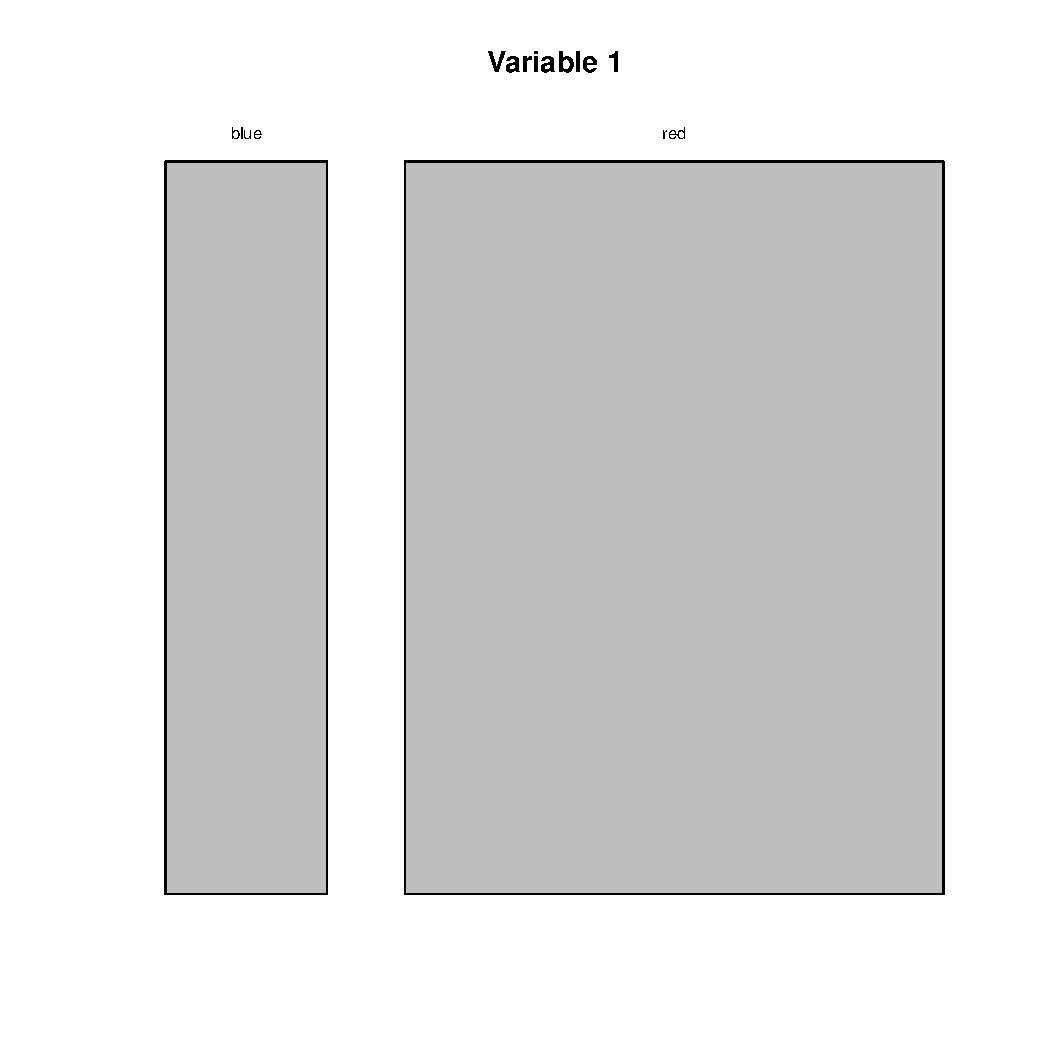
\includegraphics[scale=0.2]{mosaicPlotExample.pdf}
\end{center}
\label{fig:mosaicPlot}
\caption{\hl{something, note that code for producing this plot is available in ./latex/codeForArticle.R}}
\end{figure}

We will now build four new functions and show both how they can be used interactively and how they can be integrated with the \R{clean()} function. These four new functions are:
\begin{description}
\item[\R{isID}] A new \R{checkFunction} intended for use in the precheck-stage. This function checks whether a variable consists exclusively of long ($> 10$ characters/digits) entries that are all of equal length, as this might be personal identification codes that we do not wish to print out in the data summary.  
\item[\R{mosaicVisual}] A new \R{visualFunction} that produces so-called mosaic plots. This function will be used in the \textit{visualize} step of \R{clean()}.
\item[\R{countZeros}] A new \R{summaryFunction} that counts the number of occurrences of the value \R{0} in a variable. This function will be used in the \textit{summarize} step of \R{clean()}.
\item[\R{identifyColons}] A new \R{checkFunction} that flags variables in which values have colons that appear before and after alphanumerical characters. This is e.g. practical for identifying autogenerated interaction effects. This function will be used in the \textit{check} step of \R{clean()}. 
\end{description}
These functions are defined in turn below, and afterwards, an example of how they can be called from \R{clean()} is provided.

\subsubsection{isID - a new checkFunction without problem values}
First, let's define the \R{isID} function. As this function is not supposed to list problematic values in the variable, it falls within the category of \R{checkFunctions} represented by \R{myFullVarCheckFunction()} in the above. We do not particularly wish to use this function interactively, so we will stick to the minimal requirements of a \R{checkFunction} used in \R{check()} (see Table~\ref{table.functionTypes}). The function can then be defined by
\begin{Schunk}
\begin{Sinput}
isID <- function(v, nMax = NULL, ...) {
  out <- list(problem = FALSE, message = "")
  if (class(v) %in% setdiff(allClasses(), c("logical", "Date"))) {
    v <- as.character(v)
    lengths <- c(nchar(v))
    if (all(lengths > 10) & length(unique(lengths)) == 1) {
      out$problem <- TRUE
      out$message <- "Warning: This variable seems to contain ID codes."
    }
  }
  out
}
\end{Sinput}
\end{Schunk} 
\hl{Mention somewhere that  \R{mosiacplot()} is a base-R (\R{graphics}) function? Otherwise, it might not be completely clear, that we are passing a function name in the above...} This is essentially all we need to do in order to include this function as a precheck-function in \R{clean()}, so we will leave it as is and move on to the next function, namely \R{mosaicVisual}. 

\subsubsection{mosiacVisual - a new visualFunction}
We will define this function such that it gets the full \R{cleanR} functionality. This can be done using the code 
\begin{Schunk}
\begin{Sinput}
 mosaicVisual <- function(v, vnam, doEval) {
   thisCall <- call("mosaicplot", table(v), main = vnam, xlab = "")
   if (doEval) {
    return(eval(thisCall))
   } else return(deparse(thisCall))
 }
\end{Sinput}
\end{Schunk}
This function can now be called directly or used in \R{clean()}. We will return to its usage in \R{clean()} below. Depending on the argument \R{doEval}, either a text string with code or a plot is produced. The plot resulting from the following call is found in Figure~\ref{fig:mosaicPlot}:
\begin{Schunk}
\begin{Sinput}
mosaicVisual(toyData$var1, "variable 1", doEval = TRUE)   $
\end{Sinput}
\end{Schunk}
\hl{remove \$.}
Even though \R{mosaicVisual}, as written above, follows the style of a \R{visualFunction}, it is not yet truly one and therefore, it will not appear in a \R{allVisualFunctions()} call. In order to get this functionality, we need to change its object class. This can be done by writing
\begin{Schunk}
\begin{Sinput}
 mosaicVisual <- visualFunction(mosaicVisual, 
 				description = "Mosaic plots using graphics",
                 classes = allClasses())
\end{Sinput}
\end{Schunk}
Here, we use the function \R{allClasses()} to quickly obtain a vector of all the seven variable classes addressed in \R{cleanR}. Note that if \R{mosaicVisual} were an S3 generic function, this argument could have been left as \R{NULL} and then the classes for which methods are available would be added automatically. \hl{I'm repeating myself here, but I think it is quite a neat feature, so maybe that's okay?}

As \R{mosaicVisual} is now a full-blooded \R{visualFunction}, it will also be included in the \R{allVisualFunctions()} output table:
\begin{Schunk}
\begin{Sinput}
> allVisualFunctions()
\end{Sinput}
\begin{Soutput}
------------------------------------------------------------------------
name           description                   classes                    
-------------- ----------------------------- ---------------------------
mosaicVisual   Mosaic plots using graphics   character, Date, factor,   
                                             integer, labelled, logical,
                                             numeric                    

basicVisual    Histograms and barplots using                            
               graphics                                                 

standardVisual Histograms and barplots using                            
               ggplot2                                                  
------------------------------------------------------------------------
\end{Soutput}
\end{Schunk}
\hl{Redo this output table when makeXFunction issues are fixed.}

Now, we are done with the definition of \R{mosaicVisual} and we can turn to the next function in line, \R{countZeros}. 

\subsubsection{countZeros - a new summaryFunction}
This \R{summaryFunction} in spe is defined in the following lines of code:
\begin{Schunk}
\begin{Sinput}
countZeros <- function(v, ...) {
	res <- length(which(v == 0))
	summaryResult(list(feature = "No. zeros", result = res, value = res))
}
\end{Sinput}
\end{Schunk}
Note that as this function computes an integer (the number of zeros), there is no difference between the entires \R{\$result} and \R{\$value}. If, on the other hand, the result had been a character string, extra formatting might be required in the \R{\$result} entry (such as escaping of quotation marks), and in this scenario, the two entries would then differ. As the result is returned as a \R{summaryResult} object, a printing method is automatically called when \R{countZeros} is used interactively:
\begin{Schunk}
\begin{Sinput}
> countZeros(c(rep(0, 5), 1:100))
\end{Sinput}
\begin{Soutput}
No. zeros: 5
\end{Soutput}
\end{Schunk}
As with \R{mosaicVisual()}, we change the class of this function in order to make it appear in \R{allSummaryFunctions()} calls. But now we wish to emphasize that the function is not intended to be called on all variable types, as zeros have different roles in \R{Date}s and in \R{logical} variables:
\begin{Schunk}
\begin{Sinput}
> countZeros <- summaryFunction(countZeros,
	description = "Count number of zeros",
	classes = c("character", "factor", "integer", 
	  "labelled", "numeric"))
\end{Sinput}
\end{Schunk}
\hl{more? don't end on code.}

\subsubsection{identifyColons - a new checkFunction with problem values}
The last function mentioned above is \R{identifyColons()}. We define it using the helper function \R{messageGenerator} to obtain a properly escaped message, and we use \R{checkResult} to make its output print neatly: 
\begin{Schunk}
\begin{Sinput}
identifyColons <- function(v, nMax = Inf, ... ) {
  v <- unique(na.omit(v))
  problemMessage <- "Note: The following values include colons:"
  problem <- FALSE
  problemValues <- NULL
  
  problemValues <- v[sapply(gregexpr("[[:xdigit:]]:[[:xdigit:]]", v),
                            function(x) all(x != -1))]
  
  if (length(problemValues) > 0) {
    problem <- TRUE 
  }
  
  problemStatus <- list(problem = problem, 
                        problemValues = problemValues)
  outMessage <- messageGenerator(problemStatus, problemMessage, nMax)
  
  checkResult(list(problem = problem, 
                   message = outMessage,
                   problemValues = problemValues))
}

identifyColons <- checkFunction(identifyColons, 
    description = "Identify colons surrounded by alphanumeric characters",
    classes = c("character", "factor", "labelled"))

\end{Sinput}
\end{Schunk}
As with the previous two functions, we also change its class. Note, however, that for \R{checkFunction}s, the function description will appear in the document produced by \R{clean()} (in the \textit{Data cleaning summary} section), so now this is not only done for the sake of the \R{allCheckFunctions()} output.\\

\subsubsection{Calling the new SVC functions from clean()}
Now, we are ready to use these new functions in a \R{clean()} call. \hl{do this... what dataset should we use here? Include output in appendix, maybe.}. The extended \R{cleanR} output document should have the following modifications, relative to the standard \R{cleanR} output:
\begin{itemize}
\item We want to add the new pre-check function, \R{isID}, to the already existing pre-checks.
\item We wish to change the plot type for all variables to the new mosaic plot.
\item We want the new summary function, \R{countZeros}, to be added to the summaries performed on all variable types but \R{Date} and \R{logical}.
\item We want the new check function, \R{identifyColon}, to be added to the checks performed on \R{character}, \R{factor} and \R{labelled} variables.
\end{itemize}
These options are specified as follows:
\begin{Schunk}
\begin{Sinput}
> clean(dataSet, 
      preChecks = c("isKey", "isEmpty", "isID"),
      allVisuals = "mosaicVisual",
      characterSummaries = c(defaultCharacterSummaries(), "countZeros"),
      factorSummaries = c(defaultFactorSummaries(), "countZeros"),
      labelledSummaries = c(defaultLabelledSummaries(), "countZeros"),
      numericSummaries = c(defaultNumericSummaries(), "countZeros"),
      integerSummaries = c(defaultIntegerSummaries(), "countZeros"),
      characterChecks = c(defaultCharacterChecks(), "identifyColons"),
      factorChecks = c(defaultFactorChecks(), "identifyColons"),
      labelledCheck = c(defaultLabelledChecks(), "identifyColons"))
\end{Sinput}
\end{Schunk}
The outputted document is found in Appendix \hl{NUMTWO}. \hl{Comment. Make appendix. Remember to change dataSet to something else, when we decide what data to use here.}

\section{Something like examples}
Finally, we will present a few examples of how to make \R{cleanR} solve specific issues related to data cleaning. First, we discuss the challenges related to cleaning large datasets, particularly in terms of memory use and computation speed. Next, we show how \R{cleanR} can be used for problem-flagging. Lastly, we discuss how the \R{cleanR} output document can be included in other \R{rmarkdown} documents as a mean to produce clear and concise documentation of a dataset. \hl{I feel like there should be more topics here, but I'm all out of ideas...}

\subsection{Cleaning large datasets}
If the dataset becomes very large, the standard use of \R{clean()} outlined above might not be ideal. If there is a vast number of variables, production of the \R{rmarkdown} document might be quite slow, while an extensive amount of observations generally affects the rendering time of this document. In this section, we give a few practical examples of ways to deal with large data, while wishing to still produce (potentially very long) data cleaning overview documents. Note that the interactive tools of \R{cleanR} can be used as usual or sequentially in small subsets of the large dataset, if no such overview documents are needed. 

\subsubsection{Attacking the figures}
Though figures give a nice overview of each variable, they are also quite heavy objects in terms of memory allocation. Therefore, it might be beneficial to not include figures in the \R{cleanR} outputs for very large datasets. This is controlled via the \R{mode} argument:
\begin{Schunk}
\begin{Sinput}
> clean(toyData, mode = c("summarize", "check"))
\end{Sinput}
\end{Schunk}
If figures are indeed needed, a different approach is to choose the less memory heavy standard \R{R} figure style instead of the \R{ggplot2}\hl{reference?} figures that are the default option in \R{clean()}. This can be done using the \R{allVisuals} argument:
\begin{Schunk}
\begin{Sinput}
> clean(toyData, allVisuals = "basicVisual")
\end{Sinput}
\end{Schunk}
Of course, even less heavy plots might be achieved by writing new \R{visualFunction}s, using the guidelines from section \ref{sec:functionTemplates}. For instance, a future extension of \R{cleanR} might be the inclusion of ASCII plots, as e.g. represented in the \R{R} package \R{txtplot}\hl{reference here? It's on CRAN.}. \\

\hl{I really feel like we should do some benchmarking here, maybe just on toyData, both in terms of speed and memory use. I would make the recommendations more trustworthy and serious.}

\subsubsection{Economic memory use} 
Another solution, which is especially relevant to Windows users due to the unfortunate combination of memory control in this operating system and RStudio \hl{And also just R, right? There's got to be a nice reference on this..?}, is simply splitting the two steps performed by \R{clean}, namely producing the \R{rmarkdown} file and rendering it afterwards. If the \R{rmarkdown} file is very long, as it will typically be in very large datasets, having this file opened in memory waists precious memory capacities. Therefore, we advice users to instead split the two steps. This can be done in the following manner:
\begin{Schunk}
\begin{Sinput}
> clean(toyData, render = FALSE, openResult = FALSE}
> render("cleanR_toyData.Rmd", quiet = FALSE)
\end{Sinput}
\end{Schunk}
This also deals with the fact that \R{cleanR} can produce \R{rmarkdown} files that supersedes the upper size limit of RStudio, which is currently \hl{find number} GBs (using RStudio version 1.0.44). \hl{Is this maybe too editor specific? On the other hand, a lot of people do use RStudio...}. 

\subsection{Using cleanR for problem flagging}
If the data is large, but memory issues and computation time are less of an issue than the human time it takes to look through the data cleaning document, a viable solution might be not to include all information about all variables. Or even for more reasonably sized datasets, sometimes a brief overview of the most pressing issues can be useful. This can be achieved by using the \R{onlyProblematic} argument in \R{clean()}. By specifying \R{onlyProblematic = TRUE}, only variables that raise a flag in the checking steps will be summarized and visualized. But perhaps we are not even interested in obtaining general information about these variables, but only in getting a quick overview of the problems they might have. This can be done by also controlling the \R{mode} argument:
\begin{Schunk}
\begin{Sinput}
> clean(toyData, onlyProblematic = TRUE, mode = c("check"))
\end{Sinput}
\end{Schunk}
Now only the checking results are printed, and only for variables where problems were identified. An even more minimal output can be generated by also leaving out the checking results - then \R{clean()} essentially just produces a list of the variable names that should be investigated further:
\begin{Schunk}
\begin{Sinput}
> clean(toyData, onlyProblematic = TRUE, mode = NULL)
\end{Sinput}
\end{Schunk}
Of course, this can also be done without generating an overview document, by direct use of the \R{check()} function. When called on a \R{data.frame}, this function produces a list (of variables) of lists (of checks) of lists (or rather, \R{checkResult}s). Thus, the overall problem status of each variable can easily be unravelled using the list manipulation function \R{sapply()}: 
\begin{Schunk}
\begin{Sinput}
> toyChecks <- check(toyData)
> foo <- function(x) {
>   any(sapply(x, function(y) y[["problem"]]))
> }
> sapply(toyChecks, foo)
\end{Sinput}
\begin{Soutput}
 var1  var2  var3  var4  var5  var6 
 TRUE  TRUE  TRUE  TRUE  TRUE FALSE 
\end{Soutput}
\end{Schunk}
and we find that only the final variable, \R{var6}, for which all observations have the value \R{"Irrelevant"}, is problem-free. \hl{drop this last bit? too technical?}




\subsection{Include cleanR document in other files}
Sometimes, a \R{cleanR} document might be a useful addition to a more general overview document, including also e.g. pairwise association plots, time series plots or exploratory analysis results. To this end, it is possible to produce a \R{cleanR} document that can readily be included in other \R{rmarkdown} files. This is done by using the \R{standAlone} argument in \R{clean}, which removes the preamble from the outputted \R{rmarkdown} file. Please note, that it is still necessary to indicate which \R{rmarkdown} type is being created; the pdf and html \R{rmarkdown} styles are unfortunately not identical. 

If it is important that the embedded \R{cleanR} document can be rendered to either of these two file types, we recommend setting \R{twoCols = FALSE} and \R{output = html} in \R{clean()}, thereby essentially removing almost all output type specific formatting code from the generated \R{rmarkdown} file. 

On the other hand, if a pdf document is to be produced, a few extra lines need to be added to the preamble of the master \R{rmarkdown} document - otherwise, the two-column layout code will produce an error. The following is an example of how such a master document preamble might look like and how the \R{cleanR\_toyData.Rmd} file can then be included:
\begin{Verbatim}
---
output: pdf_document
documentclass: report
header-includes:
  - \renewcommand{\chaptername}{Part}
  - \newcommand{\fullline}{\noindent\makebox[\linewidth]{\rule{\textwidth}{0.4pt}}}
  - \newcommand{\bminione}{\begin{minipage}{0.75 \textwidth}}
  - \newcommand{\bminitwo}{\begin{minipage}{0.25 \textwidth}}
  - \newcommand{\emini}{\end{minipage}}
---

```{r, child = 'cleanR_toyData.Rmd'}
```
\end{Verbatim}
\hl{Use proper formatting here. How do we do non-R code?}

In the this example, the \R{cleanR\_toyData.Rmd} file could have been created as follows:
\begin{Schunk}
\begin{Sinput}
> clean(toyData, standAlone = FALSE)
\end{Sinput}
\end{Schunk}
and the more minimal, html-style \R{rmarkdown} file described above can be produced using
\begin{Schunk}
\begin{Sinput}
> clean(toyData, standAlone = FALSE, output = "html", twoCols = FALSE)
\end{Sinput}
\end{Schunk}
\hl{don't end on code.}


\section{Conclusion/Concluding remarks/summary/?}
\hl{Is this a thing in this journal? Otherwise, we might want to make some final remarks in the previous sections. Feels awkward to end with a bunch of code and some super specific examples...}



\appendix

\section{Appendix Something}
\includepdf[pages=2-4, pagecommand={}, frame=true, noautoscale=true, scale=0.7]{cleanR_toyData.pdf}

\section{Appendix NUMTWO}
\hl{Data cleaning with user supplied extensions here}

\end{document}
\R{characterChecks} & What checks should be performed on character variables? & \hl{what to write here?} \\
\R{factorChecks} & What checks should be performed on character variables? & \hl{what to write here?} \\
\R{numericChecks} & What checks should be performed on factor variables? & \hl{what to write here?} \\
\R{integerChecks} & What checks should be performed on integer variables? & \hl{what to write here?} \\
\R{logicalChecks} & What checks should be performed on logical variables? & \hl{what to write here?} \\ 
\R{dateChecks} & What checks should be performed on Date variables? & \hl{what to write here?} \\
\R{allChecks} & What checks should be performed on all variables (overwriting variable type specific settings if not \R{NULL})? & \R{NULL} \\

